\section{Statistical Analysis}
    \subsection{Data Preprocessing and Realized Volatility Estimation}
        In the present paper we used high-frequency data for three types of assets:
        \begin{enumerate}
            \item\textbf{Stocks}: Yandex, Sberbank, Gazprom, VTB, Moscow Exchange, Lukoil, and X5 Group;
            \item\textbf{Depositary reciepts}: Sberbank, Gazprom, VTB, and Lukoil;
            \item\textbf{Funds}: AEX, AORD, BFX, BVSP, DJI, FCHI, FTMIB, FTSE, GDAXI, GSPTSE, HSI, IBEX, IXIC, KS11, KSE, MXX, N225, OMXC20, OMXHPI, OMXSPI, OSEAX, RUT, SMSI, SPX, SSEC, SSMI.
        \end{enumerate}

        \begin{figure}[htbp]
            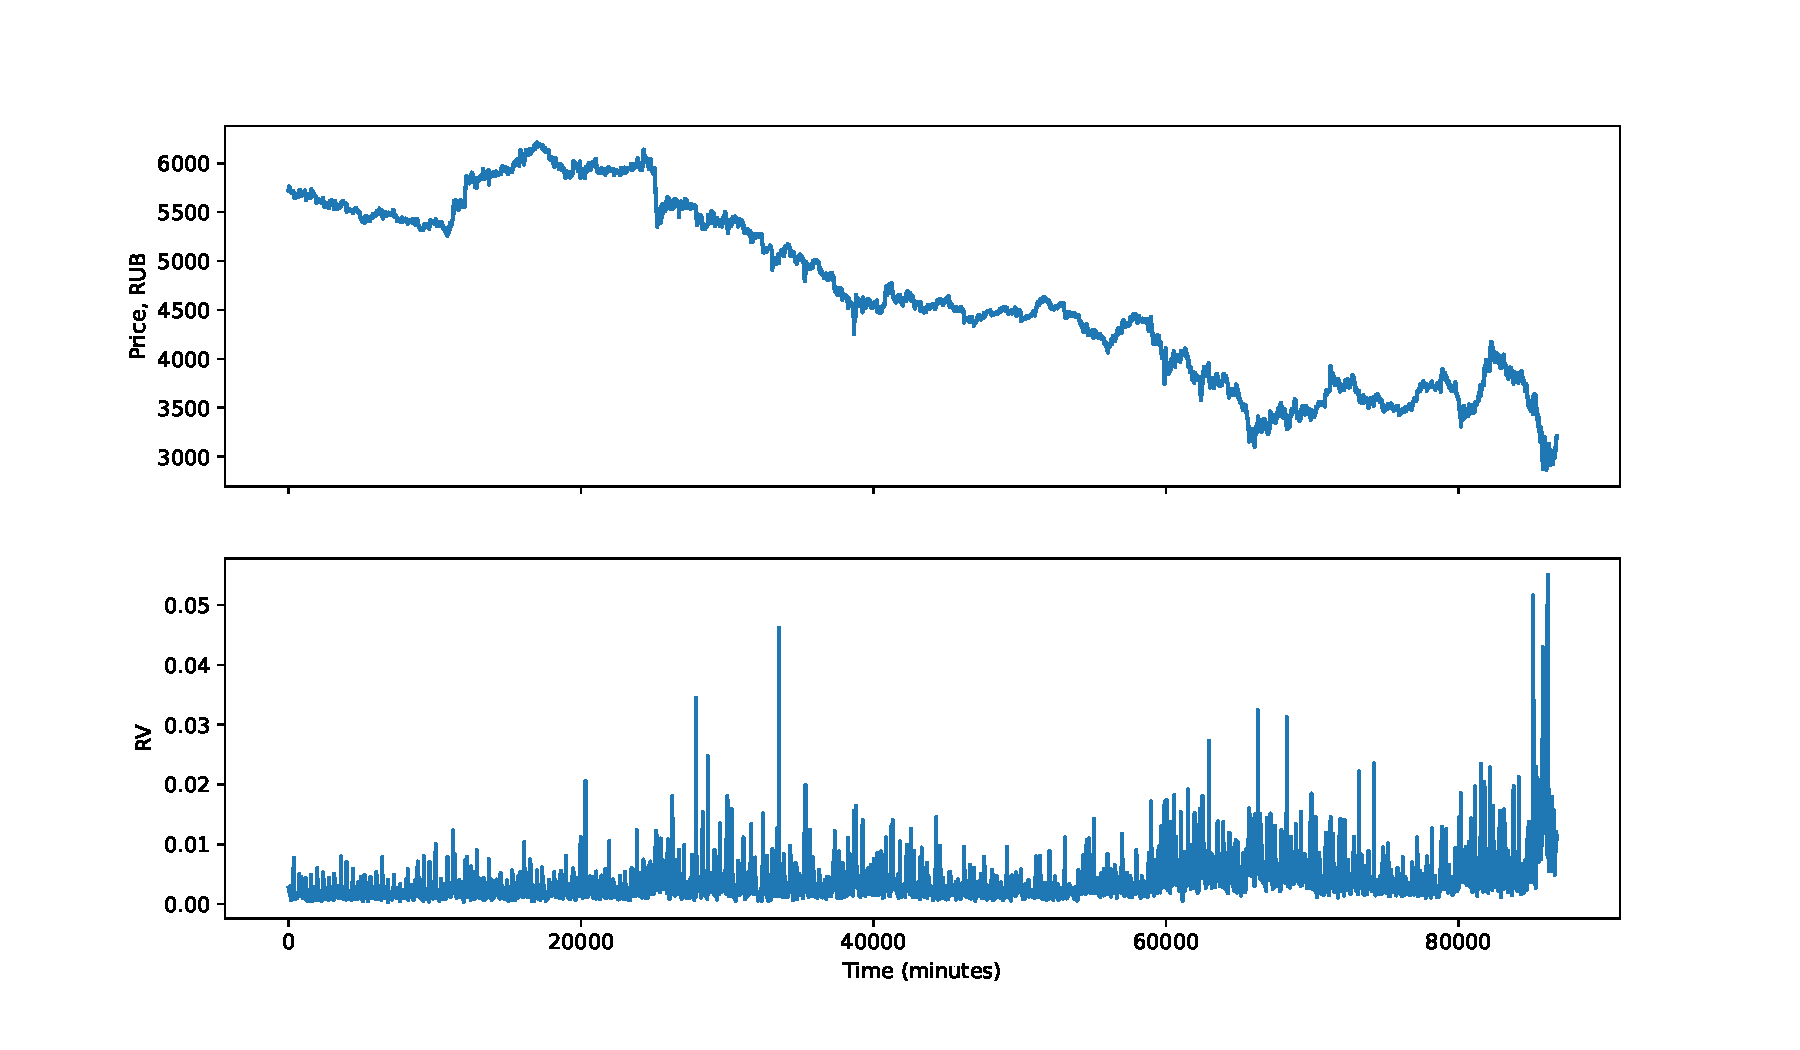
\includegraphics[width=\textwidth]{fig/YNDX RX Equity RVol.pdf}
            \caption{YNDX RX Equity. Price and Realized Volatility}
            \label{fig:priceRV} 
        \end{figure}

        Realized volatility is estimated by 15 minute disjoint windows (i.e. $\hat{RV}(t)$ is a piecewise constant function).
        Using this approach for the estimation, we can be sure that our data is correlated in the least way possible.
        We observe in the Figure \ref{fig:priceRV} that as the price decreases, the rolling mean of realized 
        volatility generally increases.
        
    \subsection{Hurst Parameter Estimation}
        \textbf{Main assumption}: for some $s_q > 0 $, $b_q > 0$ and $N = \left[\frac{T}{\Delta}\right]$ 
        (number of RV estimations via disjoint windows)
        \begin{equation}\label{eq:mainassumpt}
            N^{qs_q} m(q, \Delta) \xrightarrow[\Delta \to 0+]{} b_q.
        \end{equation}
        Under additional technical conditions equation \eqref{eq:mainassumpt} is equivalent to that the volatility process 
        belongs to the Besov smoothness space $B^{s_q}_{q, \infty}$ and for all $\tilde{s}_q > s_q$ does not belong to 
        $B^{\tilde{s}_q}_{q, \infty}$ \cite{ROSENBAUM20081434}.

        Due to the similarities in the obtained results for all assets, we shall deeply analyze the Hurst parameter estimation 
        only for the Yandex stocks (YNDX RX Equity). Plots for other equities could be found in the appendix, whereas the Hurst 
        parameter estimations for them could be found in the Table \ref{table:hurst_est}. Further in the paper we assume 
        $\Delta = 1, \dots, 40$. 
        It has been shown that under stationarity assumptions and linearity of Figure \ref{fig:logMDelta} (left)
        \begin{equation}
            \mathbb{E}\left[\left|\log\sigma_{t+\Delta} - \log\sigma_{t}\right|^q\right] = K_q \Delta^{\zeta_q},
        \end{equation} 
        and the $s_q$ does not depend on $q$. 
        In the Figure \ref{fig:logMDelta} (right) we can see that for $q = 0.6, 0.8, \text{ and } 1.0$ the dots are very discrepant for $\log\Delta > 2.0$. 
        However, we get a pretty decent linear fit for $q = 0.2$ and $q = 0.4$, therefore, the estimation on these two point would be the best one
        we can manage to extract. On the other hand, on $\zeta_q$ plot we observe a perfect linear fit for all $q$-s, therefore, $H$
        is its slope indeed.
        \begin{figure}[htbp]
            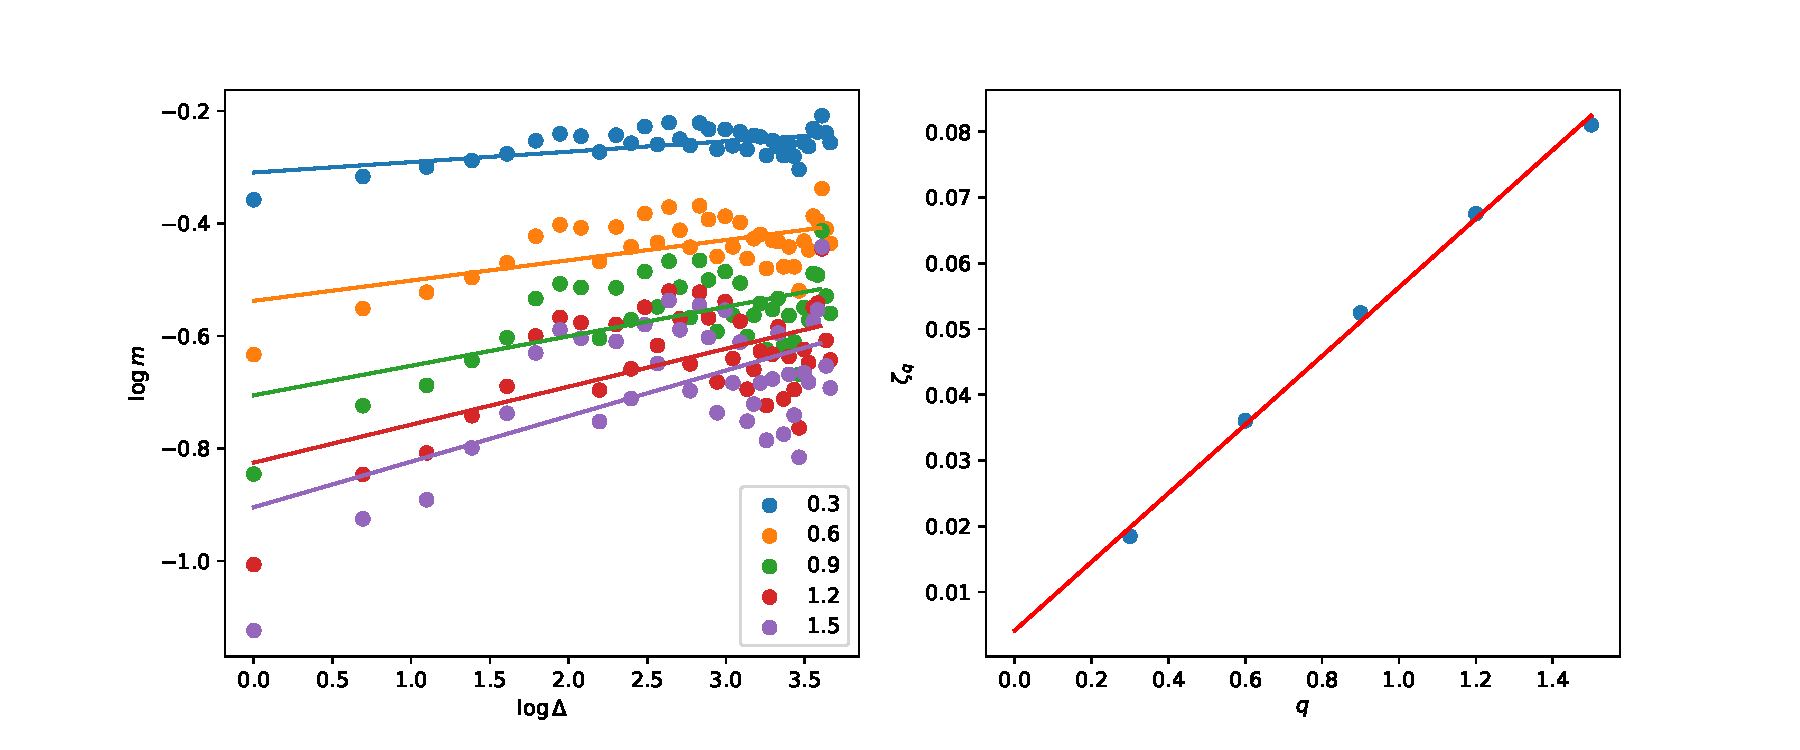
\includegraphics[width=\textwidth]{fig/YNDX RX Equity Hurst Est.pdf}
            \caption{YNDX RX Equity. Plots for $\hat{H}$}
            \label{fig:logMDelta}
        \end{figure}
        We note that the graphs for $\zeta_q$ are slightly concave, which correlates with \cite{GatheralRosenbaum2014} results.
        They conclude that this effect takes place due to the finite statistical population size.
        \begin{figure}
            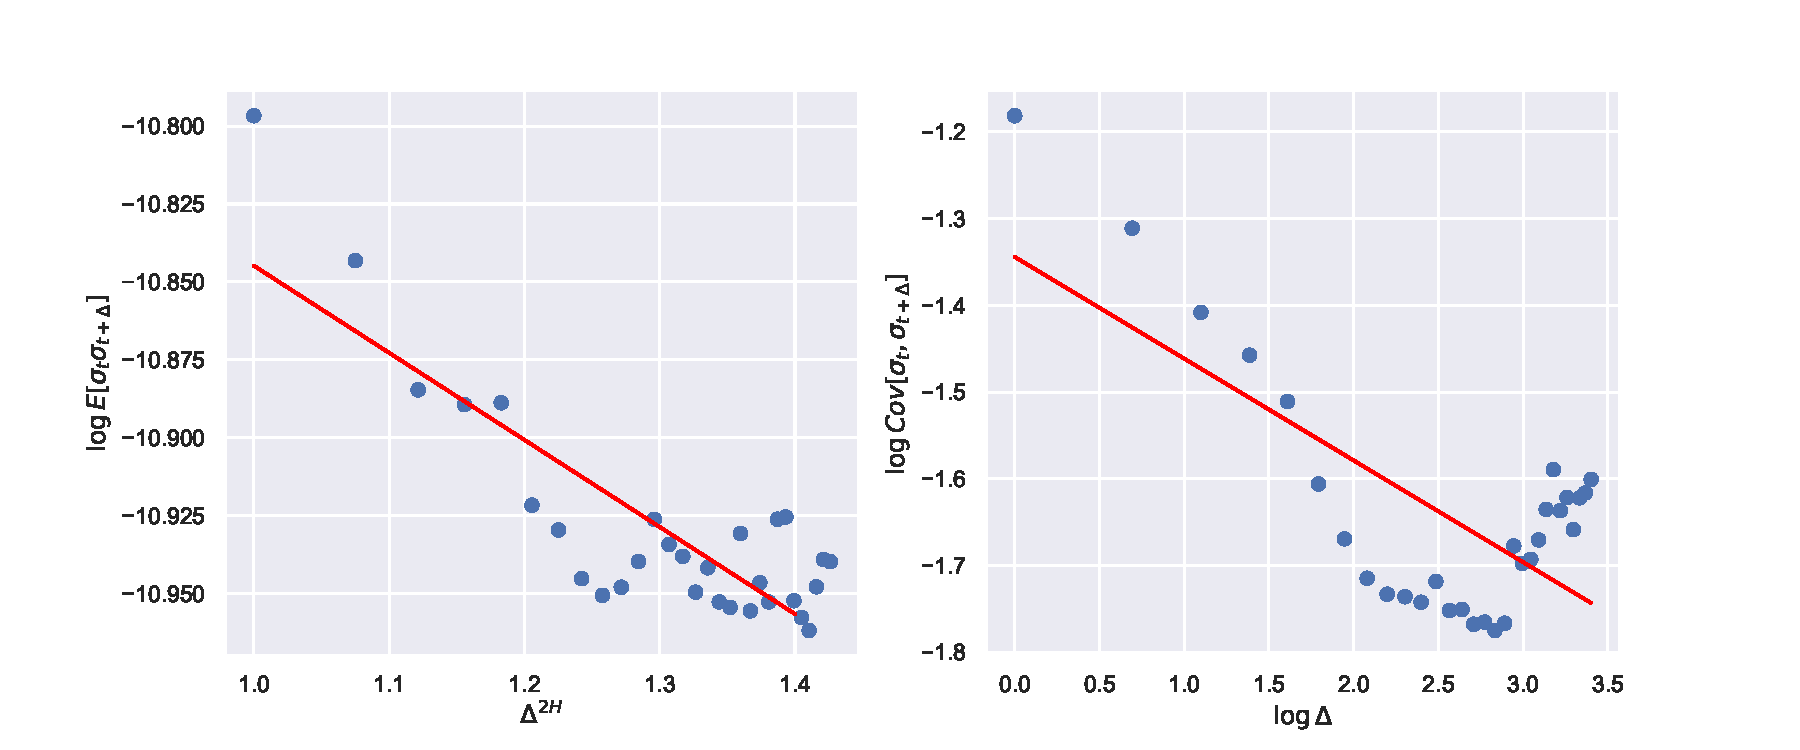
\includegraphics[width=\textwidth]{fig/YNDX RX Equity logE vs logD.pdf}
            \caption{YNDX RX Equity. Empirical counterpart of $\log\mathbb{E} \left[\sigma_{t}\sigma_{t+\Delta}\right]$ as a function of $\Delta^{2H}$ (left) and Empirical counterpart of $\log\cov [\log\sigma_{t}, \log\sigma_{t+\Delta}]$ as a function of $\log\Delta$ (right)}
        \end{figure}
        It has been proven in \cite{GatheralRosenbaum2014} that $\log\mathbb{E}[\sigma_{t}\sigma_{t+\Delta}]$ and $\log \cov[\log\sigma_t, \log\sigma_{t+\Delta}]$ are linear in $\Delta^{2H}$. And we indeed observe this behaviour in the majority of plots (especially for $\Delta < 20$, where we have enough data to work with).
        Numerical instability occurs when $\Delta$ is too large due to the lack of HF data.


        \begin{nb}
            We did not manage to obtain more HF data (only 5 months of 1m-tick data), therefore my estimations are not precise and could 
            not be used for further application.
        \end{nb}

        \begin{table}[htbp]
            \centering
            \begin{tabular}{|c|c|c|}
                \hline
                Asset Type               & Ticker & $\hat H$  \\ \hline
                \hline
                Stock                    & YNDX   & 0.0521766 \\ \hline
                Stock                    & SBER   & 0.1551646 \\ \hline
                Stock                    & VTBR   & 0.0917236 \\ \hline
                Stock                    & MOEX   & 0.0853878 \\ \hline
                Stock                    & LKOH   & 0.0730521 \\ \hline
                Stock                    & GAZP   & 0.1309705 \\ \hline
                Stock                    & FIVE   & 0.0630289 \\ \hline
                \hline
                Depositary reciept       & OGZD   & 0.0523981 \\ \hline
                Depositary reciept       & VTBR   & 0.0370185 \\ \hline
                Depositary reciept       & SBER   & 0.0578053 \\ \hline
                Depositary reciept       & LKOD   & 0.0352792 \\ \hline
                \hline
                Index                    &  AEX & 0.1271101 \\ \hline
                Index                    &  AORD & 0.0731749 \\ \hline
                Index                    &  BFX & 0.1340391 \\ \hline
                Index                    &  BVSP & 0.1285106 \\ \hline
                Index                    &  DJI & 0.1176993 \\ \hline
                Index                    &  FCHI & 0.1300797 \\ \hline
                Index                    &  FTMIB & 0.139092 \\ \hline
                Index                    &  FTSE & 0.0958701 \\ \hline
                Index                    &  GDAXI & 0.1130176 \\ \hline
                Index                    &  GSPTSE & 0.0910194 \\ \hline
                Index                    &  HSI & 0.0893922 \\ \hline
                Index                    &  IBEX & 0.1028588 \\ \hline
                Index                    &  IXIC & 0.1278909 \\ \hline
                Index                    &  KS11 & 0.1066547 \\ \hline
                Index                    &  KSE & 0.1080452 \\ \hline
                Index                    &  MXX & 0.0673153 \\ \hline
                Index                    &  N225 & 0.1063503 \\ \hline
                Index                    &  OMXC20 & 0.0997755 \\ \hline
                Index                    &  OMXHPI & 0.0954135 \\ \hline
                Index                    &  OMXSPI & 0.118664 \\ \hline
                Index                    &  OSEAX & 0.0987837 \\ \hline
                Index                    &  RUT & 0.1029421 \\ \hline
                Index                    &  SMSI & 0.1319457 \\ \hline
                Index                    &  SPX & 0.1328797 \\ \hline
                Index                    &  SSEC & 0.1170868 \\ \hline
                Index                    &  SSMI & 0.1469914 \\ \hline
            \end{tabular}
            \caption{Hurst parameter estimations}
            \label{table:hurst_est}
        \end{table}



       

    \subsection{Smoothing Effect Estimation}
        Smoothing effect is throroughly discussed in the appendix of \cite{GatheralRosenbaum2014}.

        \begin{figure}[htbp]
            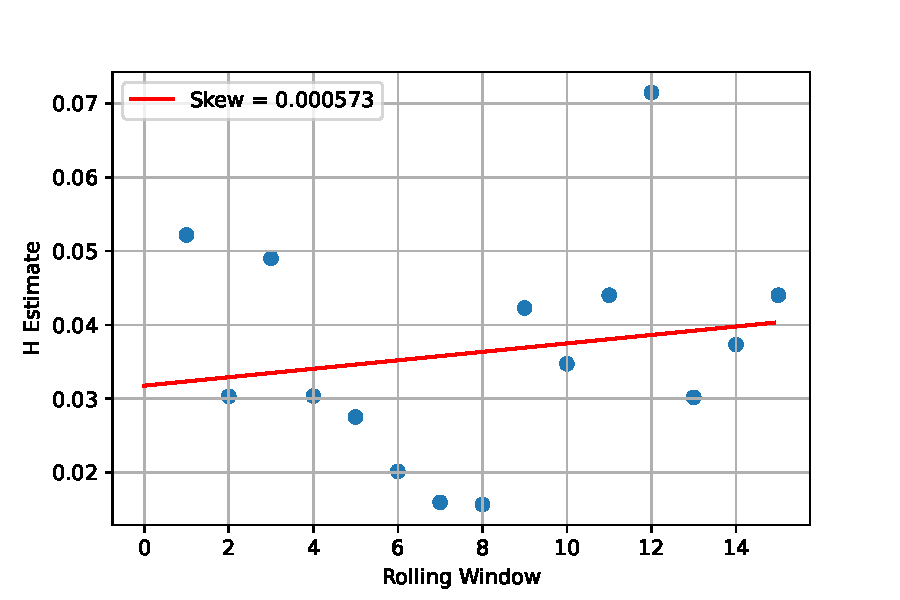
\includegraphics[width=\textwidth]{fig/YNDX RX Equity Smoothing Effect.pdf}
            \caption{YNDX RX Equity. Smoothing Effect}
            \label{fig:smooth}
        \end{figure}

        We can clearly see that due to the positive slope of the plot \ref{fig:smooth}, the hypothesis about increasing $\hat{H}$ and decreasing $\hat{\alpha}$ as $\delta$ increases is to be accepted.

    \subsection{Tests for normality of volatility's log-increments}
        In order to test the normality of the log-increments of the realized volatility, we used the following tests:
        \begin{enumerate}
            \item Visual analysis of histograms: KDE vs normal fit vs empirical fit
            \item Visual analysis of excessed kurtosis plot
            \item D'Agostino's K Squared normality test
            \item Shapiro-Wilk normality test
        \end{enumerate}

        In \cite{GatheralRosenbaum2014} the authors used \textbf{only} the visual analysis of the 
        histograms, which, as we can now say, is not surprising due to the inadequacy of results 
        for other numerical experiments.

        \subsubsection{Visual analysis of histograms and excessed kurtosis plot}
            \begin{enumerate}
                \item KDE is the \emph{kernel density estimator} of the data.
                \item \emph{Normal fit} $NF(\Delta)$ is the normal distribution fitted to the data with the same mean and variance.
                \item \emph{Empirical fit} $EF(\Delta)$ is the scaled normal distribution:
                    \begin{itemize}
                        \item $EF(1)$ is said to be same as the $NF(1)$
                        \item $EF(\Delta)$ for $\Delta > 1$ is said to be a scaled $NF(1)$ by the 
                            factor of $\Delta^{\hat{H}}$ (by this we test the monofractal scaling 
                            property of normal distribution)
                    \end{itemize}
            \end{enumerate}

            \begin{figure}[htbp]
                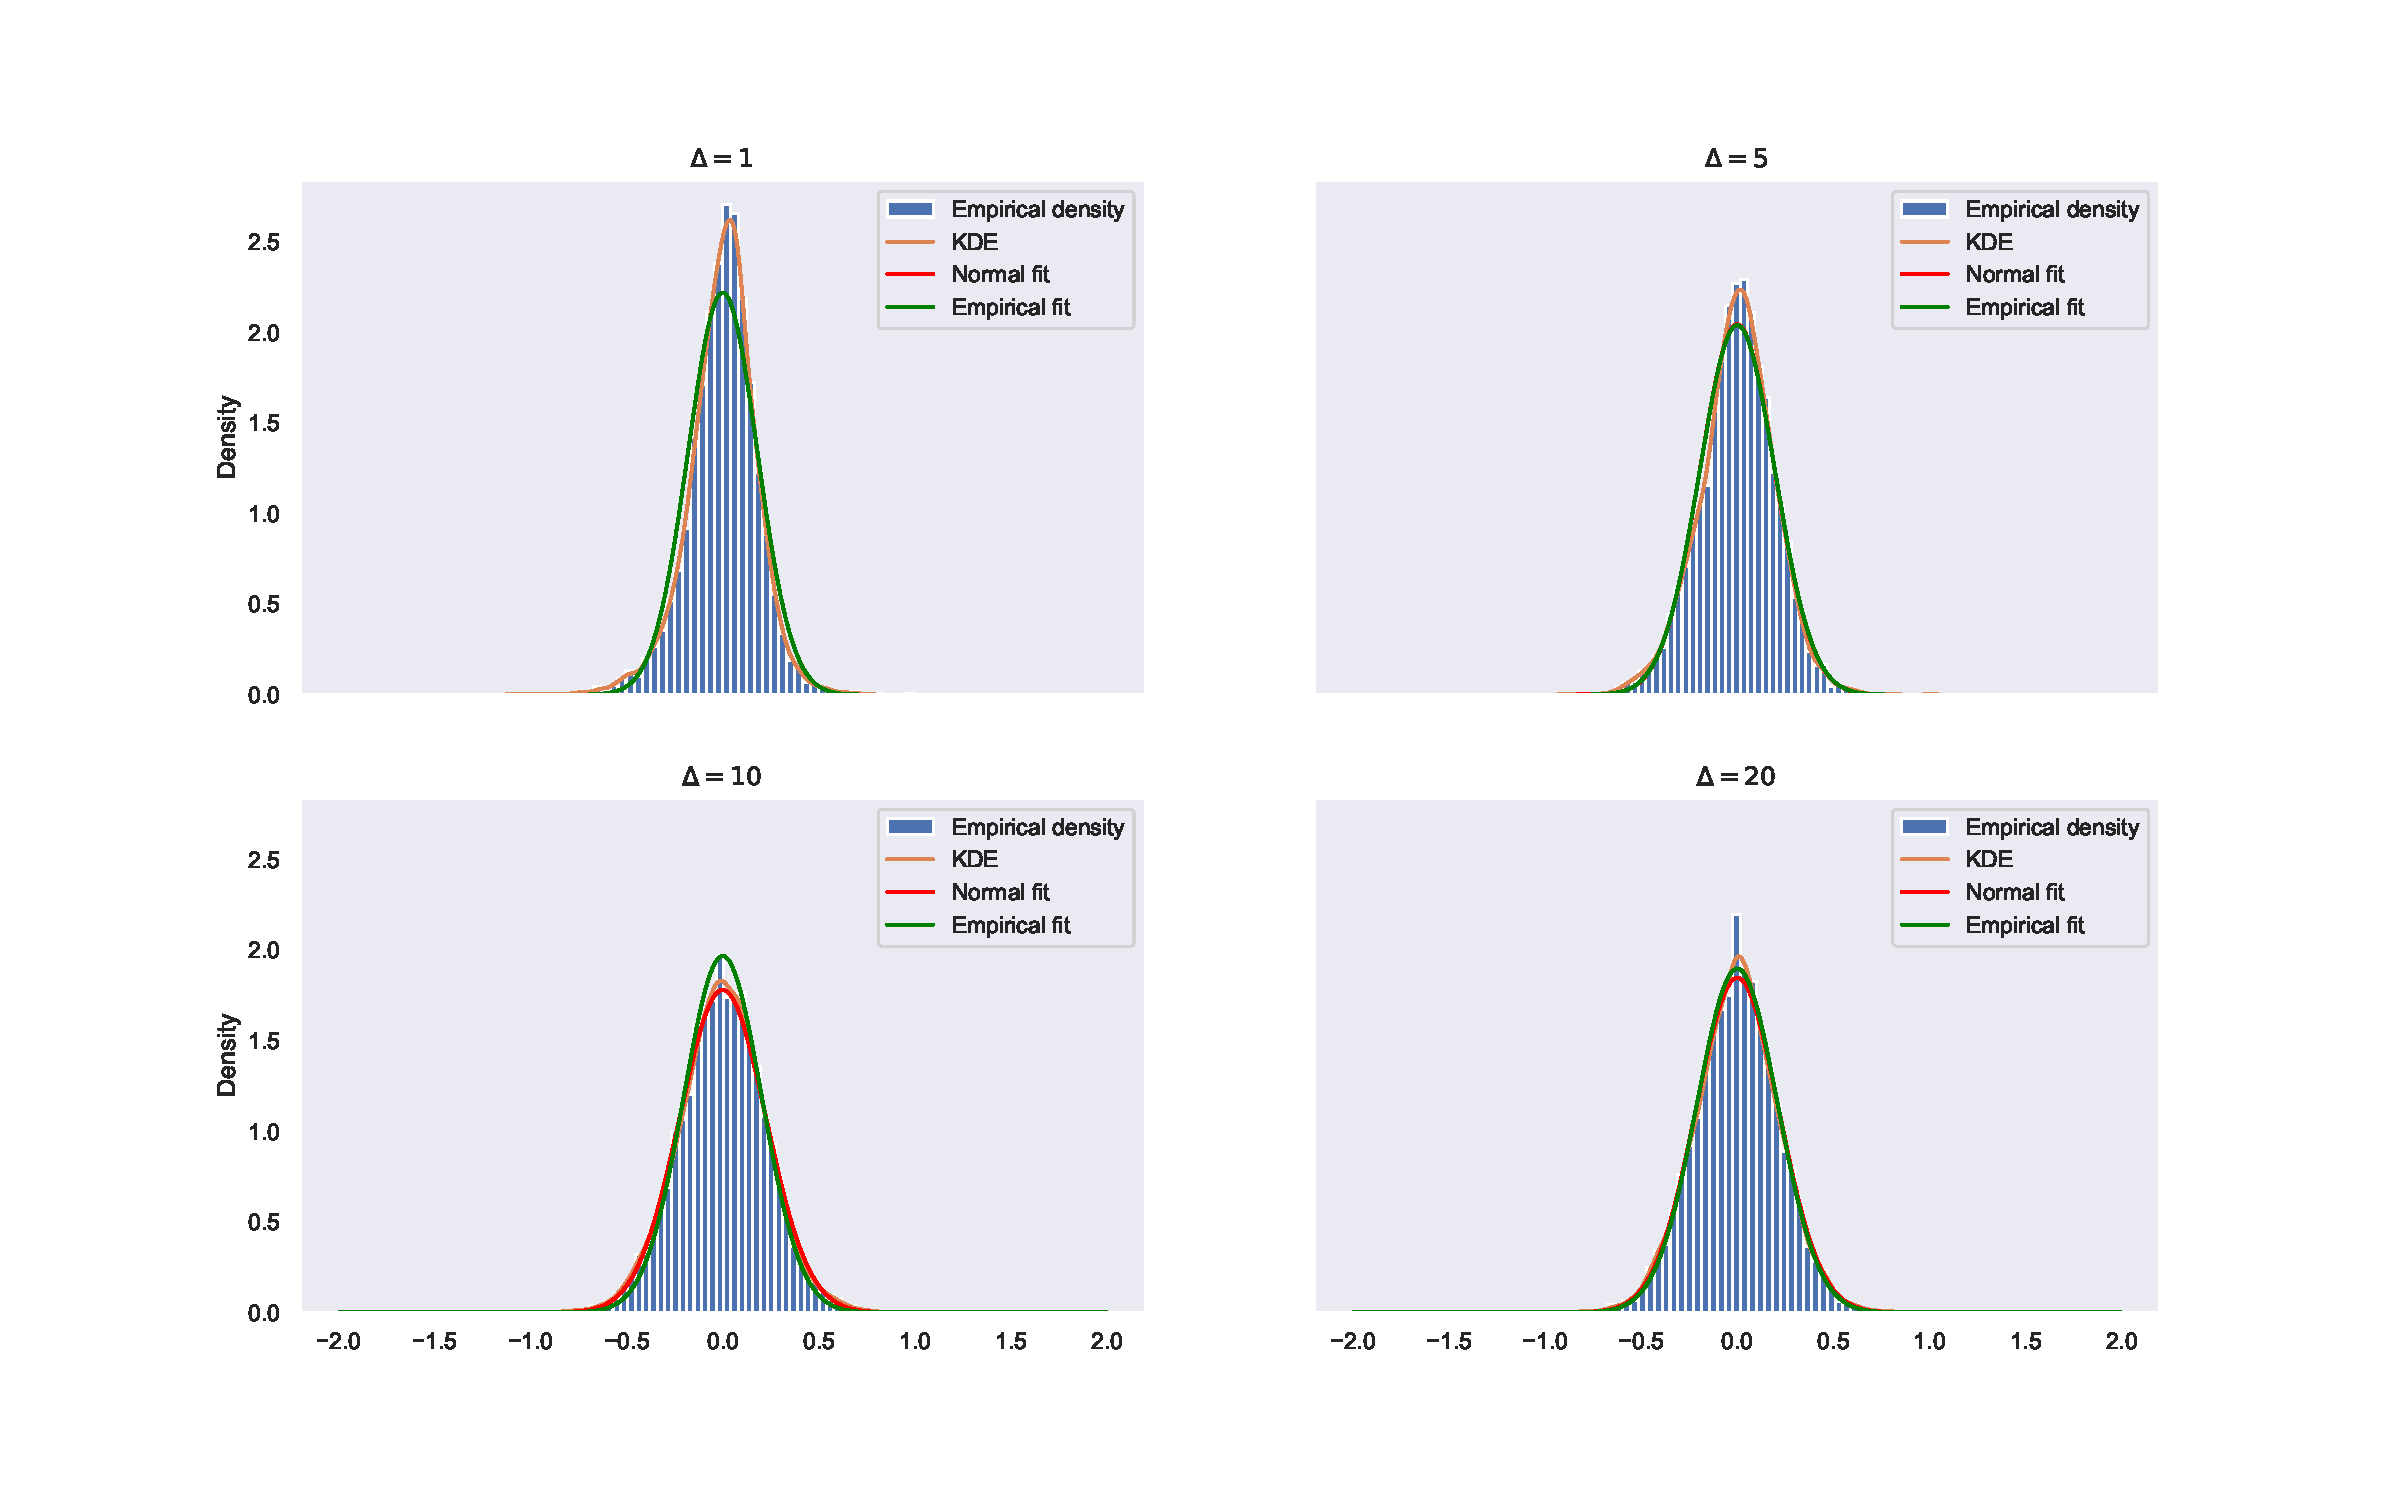
\includegraphics[width=\textwidth]{fig/YNDX RX Equity 30 Lag Hists.pdf}
                \caption{YNDX RX Equity. Empirical density of $\log \sigma_{t+\Delta} - \log \sigma_{t}$ for $\Delta = 1, 5, 10, 20$ days.}
                \label{fig:lagHists}
            \end{figure}

            Looking at the figure \ref{fig:lagHists}, we may form a conclusion: $KDE$ and $EF$ are a decent normality approximations 
            for $\Delta = 10, 20$. For others, we don't get a fancy picture: $KDE(1)$ and $KDE(5)$ have a large kurtosis 
            (they are too 'peaky' for them to be normally distributed). 
            Excessed curtosis plot \ref{fig:exkurt} confirms our visual conclusion for $KDE$ and $EF$ plots.

            \begin{figure}[htbp]
                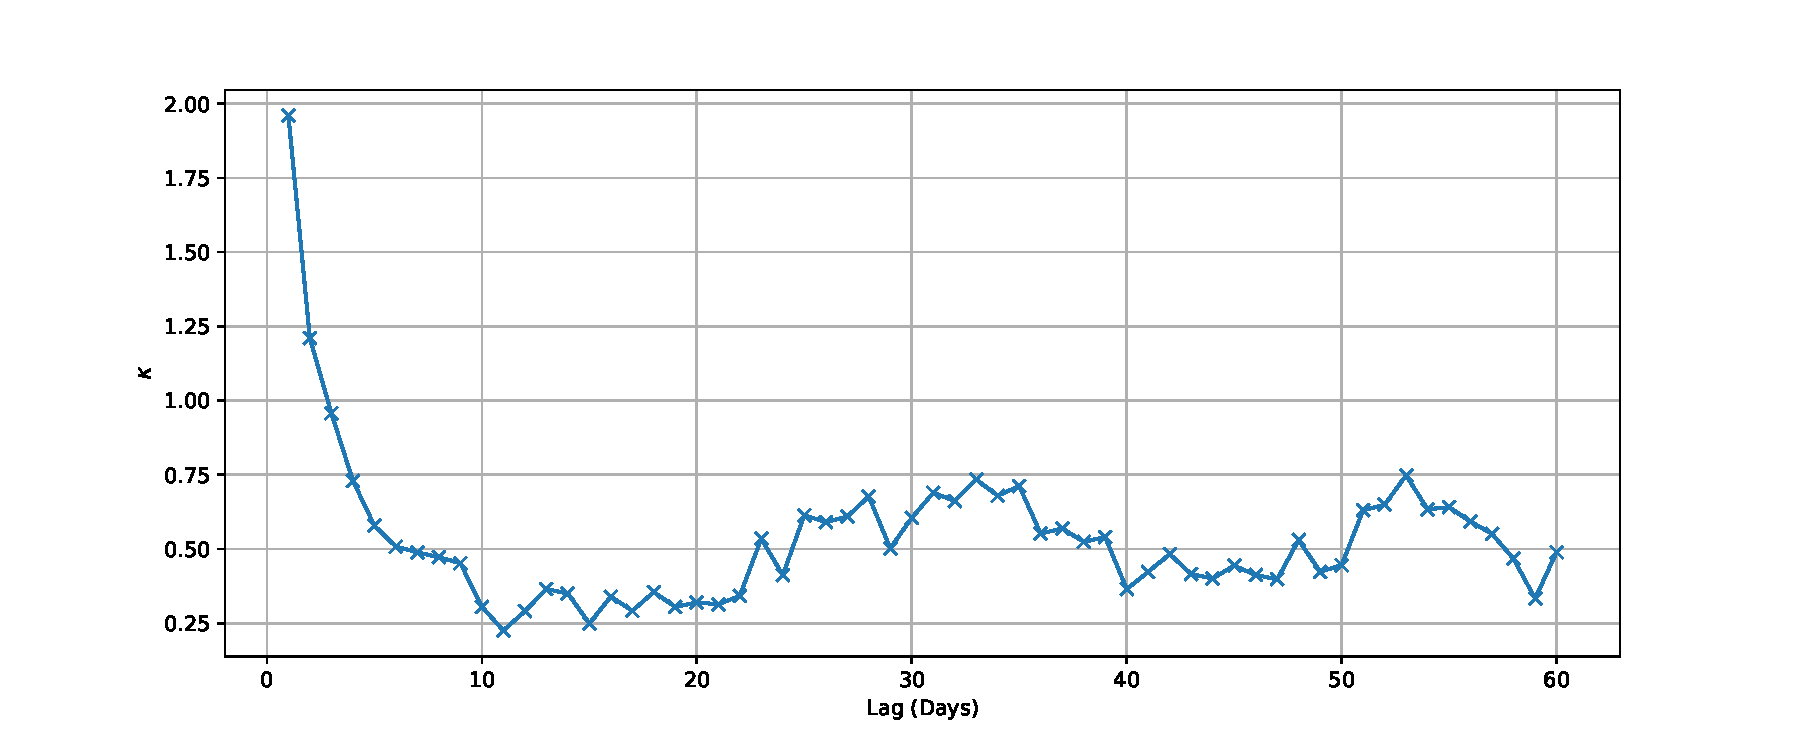
\includegraphics[width=\textwidth]{fig/YNDX RX Equity Excessed Curtosis.pdf}
                \caption{YNDX RX Equity. Excessed kurtosis $\kappa$ as a function of $\Delta$}
                \label{fig:exkurt}
            \end{figure}


        \subsubsection{Statistical tests for normality}
            We fix the confidence level to be $\alpha = 0.05$.
            \begin{nb}
                Both of these tests require the data to be independent, but we cannot guarantee this 
                due to the dependence of fBm's increments. We do our best to analyse the population,
                but these two tests give us weak proof of normality due to possible correlations.
            \end{nb}
            Looking at the tables with the results of Shapiro-Wilk and D'Agostino's K-Squared tests 
            (Tables \ref{tab:normality_tests_YNDX_} -- \ref{tab:normality_tests_LKOD_}), we can see that for the majority of lags and for the 
            majority of the considered assets, both tests showed the result "Not normal", i.e. both tests
            rejected the null hypothesis. 

            \medskip
            
            \noindent The three possible explanations are:
            \begin{enumerate}
                \item The tests are correct and the data is not normally distributed or is correlated strongly.
                \item The visual analysis of the histograms show that for many lags the KDE plot, the normal fit and 
                the empirical fit are very similar, therefore, the distribution is normal, but the data is 
                correlated strongly. The excessed kurtosis plot shows that the data is distributed very close to the normal
                distribution for $\Delta > 5$, and at its closest distance for $\Delta \in [10, 22]$.
                \item We get a population sampling error (not enough data).
            \end{enumerate} 